\documentclass{beamer}
\usepackage[ngerman]{babel}
\usepackage[utf8]{inputenc}
\usepackage{csquotes}
\usepackage{url}
\usepackage{graphicx}
\usepackage{amsmath}
\usepackage{amssymb}
\usepackage{nicefrac}
\usepackage{eurosym}
\usepackage{xcolor}
\usepackage{alltt}
\usepackage{tikz}
\usepackage{ragged2e} 
\usepackage{tabu}
\usetikzlibrary{trees}
\usepackage{calc,color,colortbl,nicefrac}
\newtheorem*{bem}{Bemerkung}
\usepackage{multirow}


%smaller footnotes
\renewcommand{\footnotesize}{\tiny}
%reduce spacing in footnotes
\setlength{\footnotesep}{0em}

%use for inline citation formatting
\newcommand{\textct}[1]{{\textsuperscript{\tiny \color{gray}#1}}}

\newlength{\myX}
\newlength{\myY}

%absolute figure positioning
\usepackage[absolute,overlay]{textpos}
  \setlength{\TPHorizModule}{1mm}
  \setlength{\TPVertModule}{1mm}

%quote environment with reference 
\def\signed #1{{\leavevmode\unskip\nobreak\hfil\penalty50\hskip2em
  \hbox{}\nobreak\hfil(#1)%
  \parfillskip=0pt \finalhyphendemerits=0 \endgraf}}
\newsavebox\mybox
\newenvironment{aquote}[1]
  {\savebox\mybox{#1}\begin{quote}}
  {\signed{\usebox\mybox}\end{quote}}

\definecolor{purp}{HTML}{3333b3}
\definecolor{dgrey}{rgb}{0.8,0.8,0.8}
\definecolor{bgrey}{rgb}{0.95,0.95,0.95}

\usepackage{graphicx}
\graphicspath{{img/}}

\newlength{\stdlength}
% Standardlaenge fuer Skript und Folien
\setlength{\stdlength}{8cm}

\usetheme{Copenhagen}
\usefonttheme{professionalfonts}
\usecolortheme{crane}

\bibliography{literature}
\usepackage[style=authoryear, backend=bibtex]{biblatex} 
\addbibresource{literature.bib}

\defbibenvironment{bibliography}
{\list{}
{\setlength{\leftmargin}{\bibhang}%
\setlength{\itemindent}{-\leftmargin}%
\setlength{\itemsep}{6px}%
\setlength{\parsep}{\bibparsep}}}
{\endlist}
{\item \scriptsize}

\definecolor{mygrey}{RGB}{80,80,80}

\setbeamertemplate{headline}
{%
\hfill
\textbf{\insertsection} \
\insertsubsection \
\insertframenumber / \inserttotalframenumber
}
\setbeamertemplate{navigation symbols}{}

\title{Informationsvisualisierung}
\subtitle{Übung 1}
\author{
Frank Rosner
}

\institute{
Martin-Luther-Universität Halle-Wittenberg
}
\date{WS 13/14}

\begin{document}

\frame{\titlepage}

\section{Aufgabe 1.1}

\begin{frame}{Definition / Beispiel Scatterplot}
\begin{textblock}{80}(50,40)

\end{textblock}
\textbf{Scatterplot (Streudiagramm)}
\begin{itemize}
\item Darstellung mehrerer Variablen in Koordinatensystem
\item Visualisierungen von Abhängigkeiten
\end{itemize}
\begin{center}
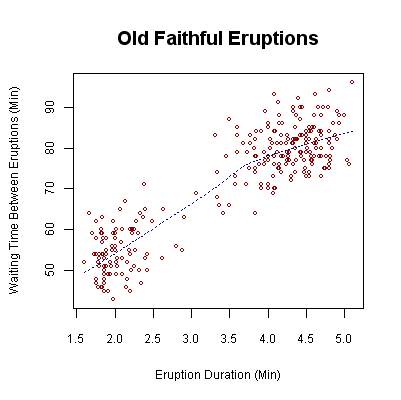
\includegraphics[width=5.5cm, trim=1.5cm 2cm 1cm 2cm, clip=true]{Oldfaithful3.png}
\end{center}
\vspace*{-1em}
\end{frame}

\section{Aufgabe 1.2}

\begin{frame}{Scatterplot der Fahrzeugdaten}
\textbf{Offensichtliche Korrelation}
\begin{center}
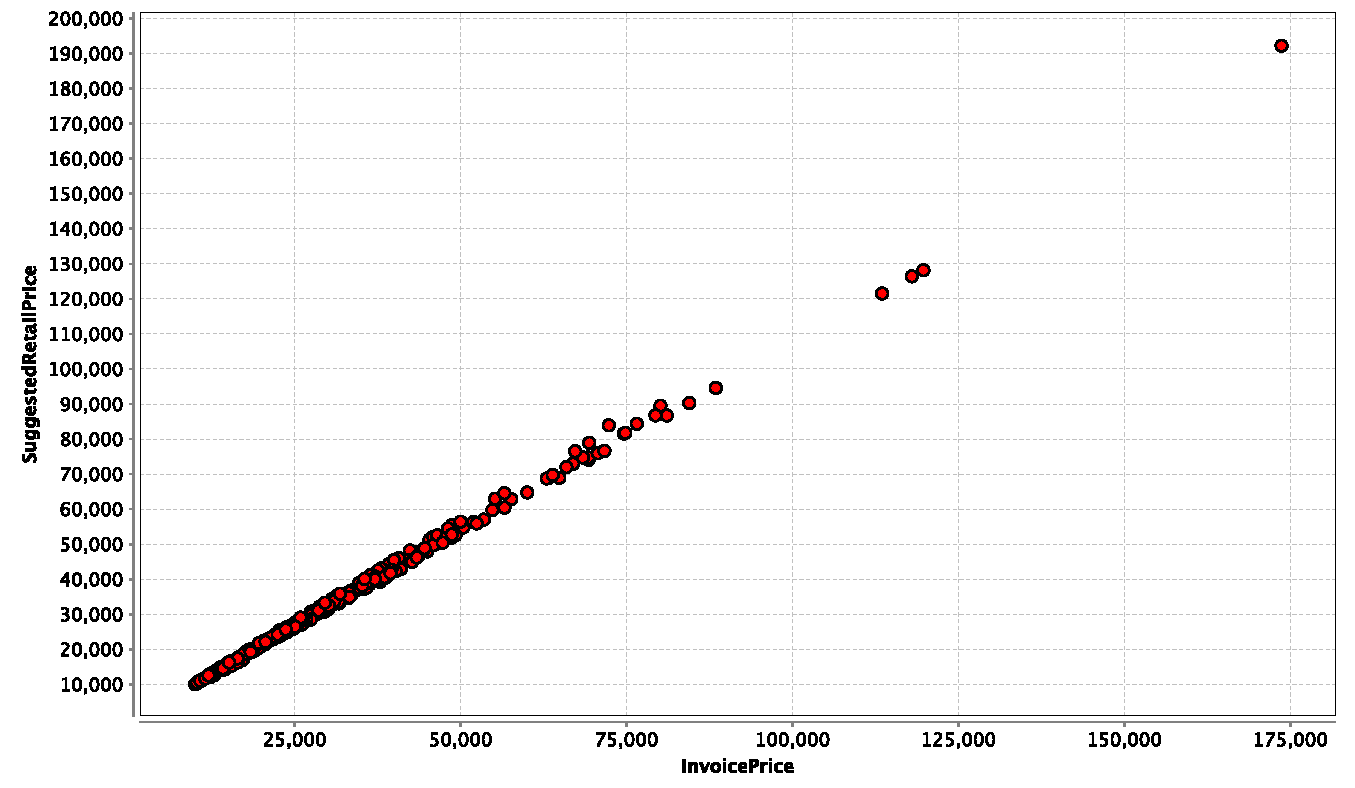
\includegraphics[width=1\linewidth]{U1_InvoicePrice_SuggestedRetailPrice.pdf}
\end{center}
\end{frame}

\begin{frame}{Hypothese auf Fahrzeugdaten}
\begin{onlyenv}<1->\textbf{Hypothese:} Größere Autos sind schwerer\end{onlyenv} \begin{onlyenv}<2->$\Rightarrow$ stimmt\end{onlyenv}
\begin{onlyenv}<1->\begin{center}
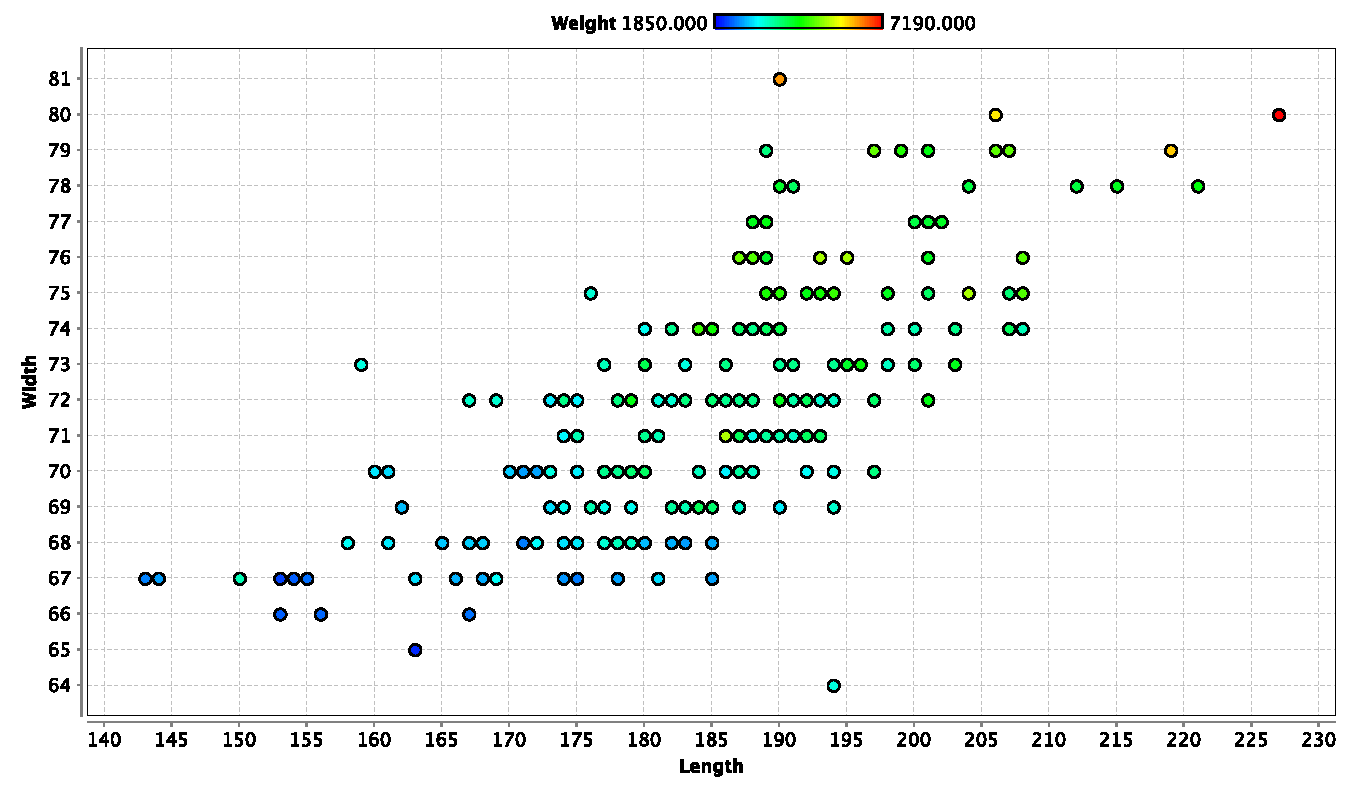
\includegraphics[width=1\linewidth]{U1_Length_Width_Weight.pdf}
\end{center}
\end{onlyenv}
\end{frame}




\end{document}